In this work, we will investigate alcohol-water mixtures of 8 different 
alcohols with the solution concentrations varying from 2\% to 50\% for each.
The investigated alcohols include:\\
- ethylene glycol\\
- ethanol\\
- methanol\\
- glycerol\\ 
- 1-propanol\\
- 2-propanol\\ 
- 1,3-propanediol\\
- propylene glycol\\
as they are alcohol types that were used as industrial antifreeze.
The methodology is operated according to the following diagram
\begin{figure}
    \begin{center}
        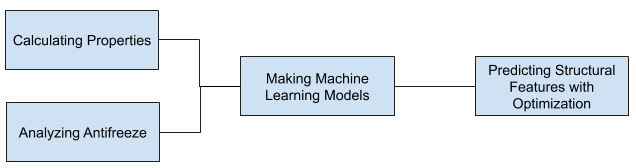
\includegraphics[width=1\textwidth]{method.png}
    \end{center}
    \caption{Procedure of the Methodology}
\end{figure}
\section{Calculating Properties}
In this work, the calculations of properties are carried out by LAMMPS \cite{plimpton_fast_1995}.
Since the investigated objects are water-alcohol mixtures, the fundamental inputs include\\
- Number of alcohol molecules\\
- Number of water molecules\\
- Declaring implemented alcohol molecular model\\
- System temperature T\\
- System volume V\\
- System pressure P\\
TIP4P/Ice \cite{abascal_potential_2005} will be used as the water model throughout all 
mixtures while all alcohol models are based on OPLS-AA \cite{jorgensen_development_1996}, 
which is derived from the Optimized Potentials for Liquid Simulations models 
\cite{jorgensen_opls_1988}.The system pressure is set at 1 atm while the volume of the 
system is set at 40x40x40 $\textup{\AA}^3$ throughout all simulations.\\
Since we are investigating throughout the mass concentration of mixtures, 
we construct a small converter that approximate the number of alcohol 
molecules and water molecules from input mass concentrations. Assuming 
that the sum of volume of water and volume of alcohol equals the system 
volume, we obtain the following:
\begin{equation}
    m_{w}=\rho_{w} V_{w}
\end{equation}
\begin{equation}
    m_{w}=\rho_{w}\left(V-V_{a l c}\right)
\end{equation}
\begin{equation}
    m_{w}=\rho_{w}\left(V-m_{a l c} / \rho_{a l c}\right) \label{eq:1}
\end{equation}
Where $m_w$ is mass of water, $\rho_w$ is density of water, $V_w$ is volume 
of water, $m_{alc}$ is mass of alcohol, $\rho_{alc}$ is density of alcohol and
$V_{alc}$ is volume of alcohol.\\
But then the mass concentration is:
\begin{equation}
    c_{\%}=\frac{m_{alc}}{m_{a k}+m_{alc}}
\end{equation}
Thus
\begin{equation}
    m_{alc}=\frac{c_{\%}}{1-c_{\%}}m_w  \label{eq:2}
\end{equation}
Substitute \ref{eq:2} into \ref{eq:1} we obtain
\begin{equation}
    m_{w}=\rho_{w}\left(V-\frac{c_{\%}}{1-c_{\%}} m_{w} / \rho_{a l c}\right)
\end{equation}
Collect all the terms that contain $m_w$ into one side then eliminate the coefficients, we obtain:
\begin{equation}
    m_{w}=V \rho_{a l c} \rho_{w}\left(1-c_{\%}\right) /\left(\rho_{w} c_{\%}+\left(1-c_{\%}\right) \rho_{a l c}\right)
\end{equation}
\begin{equation}
    m_{a l c}=\frac{1-c_{\%}}{c_{\%}} m_{w}
\end{equation}
Thus, the number of alcohol molecules $N_{alc}$ and the number of water molecules $N_w$
can be obtained as follows:
\begin{equation}
    N_{a l c}=N_{A} \frac{m_{a l c}}{M_{a l c}}
\end{equation}
\begin{equation}
    N_{w}=N_{A} \frac{m_{w}}{M_{w}}
\end{equation}
Furthermore, $N_A$ is the Avogadro number, $M_{alc}$ is the molar mass of alcohol and 
$M_w$ is the molar mass of water.

The method is validated by taking the calculated number of molecules to 
calculate the mass concentration. The error between calculated mass 
concentrations and input concentrations do not surpass 2\%. Thus, the method 
is valid. The error arises from the fact that an integer number of molecules 
is required.\\
The densities of pure liquid are taken from online chemistry database CHERIC 
(Chemical Engineering and Materials Research Information Center) under 
conditions of 1 atm and 293K. Thus, the temperature of systems are set at 
293K and 1 atm pressure.\\
The thermal conductivity can be deconstructed into 2 terms: virial and 
convective. The virial terms represents the interatomic interaction 
contribution to the thermal conductivity while the convective terms show the 
diffusion in the thermal conductivity. It is shown that the virial terms 
dominate the convective terms and can be used to represent the trend of 
values \cite{lin_constructing_2011}. Furthermore, in LAMMPS, the calculation time of 
the virial terms is much shorter compared to the total thermal conductivity 
due to the absence of the enthalpy quantity that is required to calculate the 
total term. Since the main aim of this work is the trend of values instead of 
the absolute values themselves, to reduce calculation costs, only the virial 
term is calculated. However, we can still calculate the total terms for 
viscosity since we do not need enthalpy quantity for viscosity calculations.


\section{Analyzing Antifreeze Molecules}
Since the purpose is to make a function of structural features to desired 
properties, in this section, we will discuss about which features should be 
chosen as variables for the functions. The variables’ roles are not only to 
form relationships to desired properties, but also to distinguish different 
data points. To avoid unnecessary complexity, the variables (or structural 
features) should be independent.

In alcohol, it is already understood that the number of OH groups 
significantly affect the ability of heat transfer while the position of the OH 
group also change the properties values \cite{manjunatha_investigation_2017}. However, there 
might be also other potential structural features that are left uninvestigated. 
Since we only care about the impact of the structural features on the 
thermophysical properties, we will select all the features that define an 
alcohol molecular structure.
\newpage
\begin{figure}[h!]
    \centering
    \begin{subfigure}[b]{0.3\linewidth}
      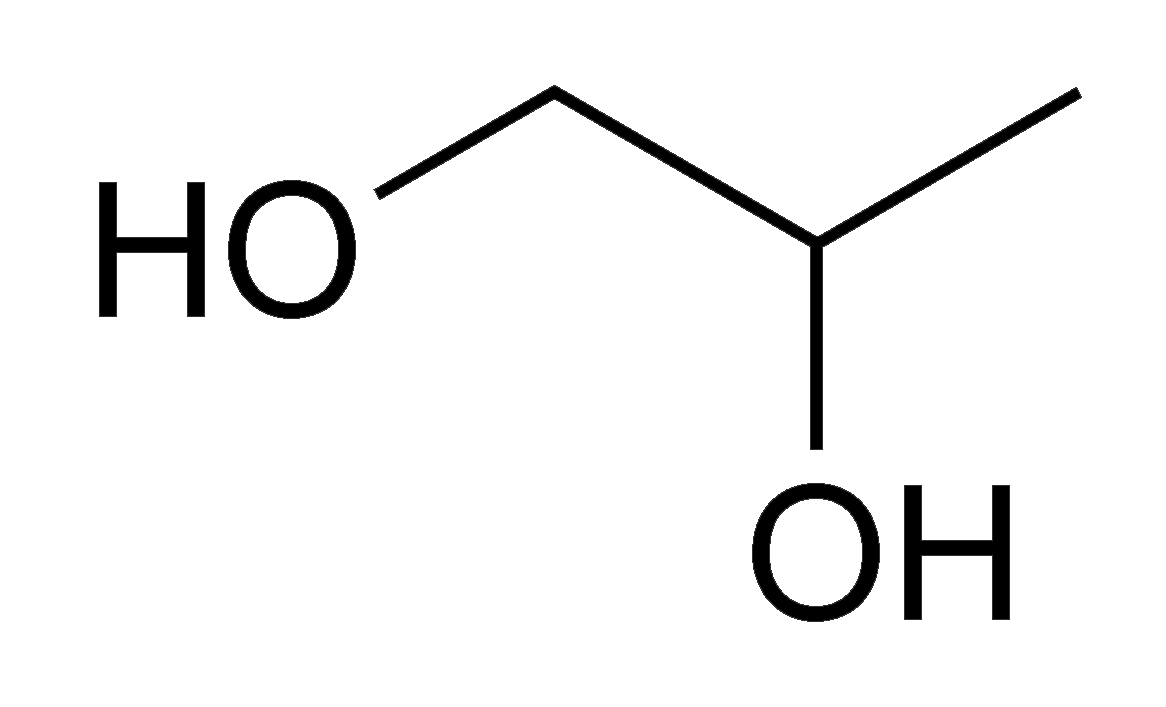
\includegraphics[width=\linewidth]{prplene.png}
       \caption{Propylene Glycol}
    \end{subfigure}
    \begin{subfigure}[b]{0.3\linewidth}
      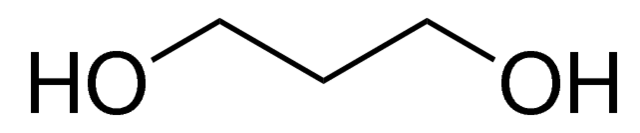
\includegraphics[width=\linewidth]{13prop.png}
      \caption{1,3-propanediol}
    \end{subfigure}
    \begin{subfigure}[b]{0.3\linewidth}
        
\includegraphics[width=\linewidth]{glycerol.png}
        \caption{Glycerol}
      \end{subfigure}
    \begin{subfigure}[b]{0.3\linewidth}
      
\includegraphics[width=\linewidth]{1prop.png}
      \caption{1-propanol}
    \end{subfigure}
    \begin{subfigure}[b]{0.3\linewidth}
      
\includegraphics[width=\linewidth]{2prop.png}
      \caption{2-propanol}
    \end{subfigure}
    \begin{subfigure}[b]{0.3\linewidth}
        
\includegraphics[width=\linewidth]{ethlne.png}
        \caption{Ethylene Glycol}
      \end{subfigure}
      \begin{subfigure}[b]{0.3\linewidth}
        
\includegraphics[width=\linewidth]{meth.png}
        \caption{Methanol}
      \end{subfigure}
      \begin{subfigure}[b]{0.3\linewidth}
        
\includegraphics[width=\linewidth]{ethanol.png}
        \caption{Ethanol}
      \end{subfigure}
    \caption{ Molecular Structures of Sample Alcohol Types}
    \label{fig:mol}
\end{figure}
As we can see, there are not many significant differences and are a lot of 
similarities across the molecular structures of all the selected alcohols. 
Thus, to distinguish different alcohols, the following features (in a 
molecular structure) will be used:\\
- Number of oxygen atoms\\
- Number of carbon atoms\\
- Number of single bonds, which also represents the number of hydrogen atoms\\
- The length of the main carbon chain\\
- The position(s) of the hydroxyl group(s)\\
To differentiate between different mixtures, the following features will be used:\\
- Number of water molecules\\
- Number of alcohol molecules\\
We can also see that glycerol is the only alcohol type that possess 3 hydroxyl 
groups while propylene glycol is really close to 1,3-propanediol 
(only different in the position of the 2nd hydroxyl group). Meanwhile, 
ethanol is quite similar to methanol and 1-propanol is a structural isomer 
of 2-propanol. Interestingly, among all the above alcohol types, methanol 
is the only type that is less viscous than water.

\section{Machine Learning Implementation}
Two sets of data will be prepared: a training data set and a testing data set. 
The training data set is used to construct the model while the testing data 
set is left unused throughout the training process and only used in 
approximating the true error so that the model is not overfit. We will make 
a model of thermal conductivity and a model of viscosity.

The parameter set for each model are decided by using k-fold methods. 
Within the possible range of parameters, every combination of parameters 
is cross-validated using the k-fold methodology and then the training 
performance scores are compared. The parameter set of the model that has 
the best training performance score will be chosen.
The selected parameter sets will be used to create the models with the 
training data set. The constructed models will then be tested on the 
testing data set to obtain the performance score. 

To thoroughly analyze the machine learning implementation, the training 
data set and testing data set will be decided by 2 ways: 
random and out of sample.
The random method is to randomly divided the entire data set into the 
training data set and the testing data set and create the models. 
The resulting models will be used to progress to the final step.
The out of sample method is to completely exclude an alcohol type out of 
the training sample. Four alcohol types, namely propylene glycol, methanol. 
2-propanol and glycerol, will be in turn excluded to assess the 
characteristics of machine learning approach in this problem.

The performance score of the testing and training processes will be 
calculated using the $R^2$ score method as follows:
\begin{equation}
    R^{2}=1-\frac{S S R}{T S S}
\end{equation}
Where
\begin{equation}
    S S R=\sum_{i=1}^{n}\left(y_{i}-f\left(x_{i}\right)\right)^{2}
\end{equation}
\begin{equation}
    T S S=\sum_{i=1}^{n}\left(y_{i}-\frac{1}{n} \sum_{j=1}^{n} y_{j}\right)^{2}
\end{equation}
Furthermore, SSR stands for squared sum of residual, TSS stands for total squared sum, 
y is the real value, $f(x_i)$ is the predicted value, n is the number of data in 
the data sample and i and j are data indices.
\section{Optimization}
In the optimization step, I will find the optimal values of desired properties 
while returning the corresponding inputs, which is the structural features in 
this work. The finding is done by setting up an optimization problem with an 
objective function and different constraints. The objective function guides 
the computer to find the optimal results while the constraints help us to 
remove the unrealistic outcomes.\\
This work considers optimization of thermal conductivity and viscosity. 
Thus, the problem will be described as follows:\\
Maximize:
\begin{equation}
    \alpha \frac{T C-\overline{T C}}{\sigma_{T C}}-\beta \frac{V i s c-\overline{V i s c}}{\sigma_{V i s c}}
    \label{eq:obj} 
\end{equation}
Subject to:\\
- The number of alcohol molecules $>$ 0\\
- The number of carbons and oxygens $>$ 0\\
- The position of OH groups $>$ 0\\
- The length of the main carbon chain $<$ the number of carbons\\
- The number of total molecules $<$ 2100 (estimated number that fits in the investigated volume)\\
- Every input is integer\\
Where $\alpha$ and $\beta$ are the weighting factors that define the importance of the 
thermal conductivity and viscosity. In this research, we value the thermal 
conductivity and the viscosity equally, which means $\alpha=\beta=1$. $\sigma_{T C}$ is the standard 
deviation of the sample thermal conductivity values, $\sigma_{Visc}$ is the standard 
deviation of the sample viscosity values, $\overline{T C}$ is the mean of the sample 
thermal conductivity values and $\overline{V i s c}$ is the mean of the sample viscosity 
values. The values of thermal conductivity and viscosity will be first 
standardized before processed in the objective function \ref{eq:obj}.



